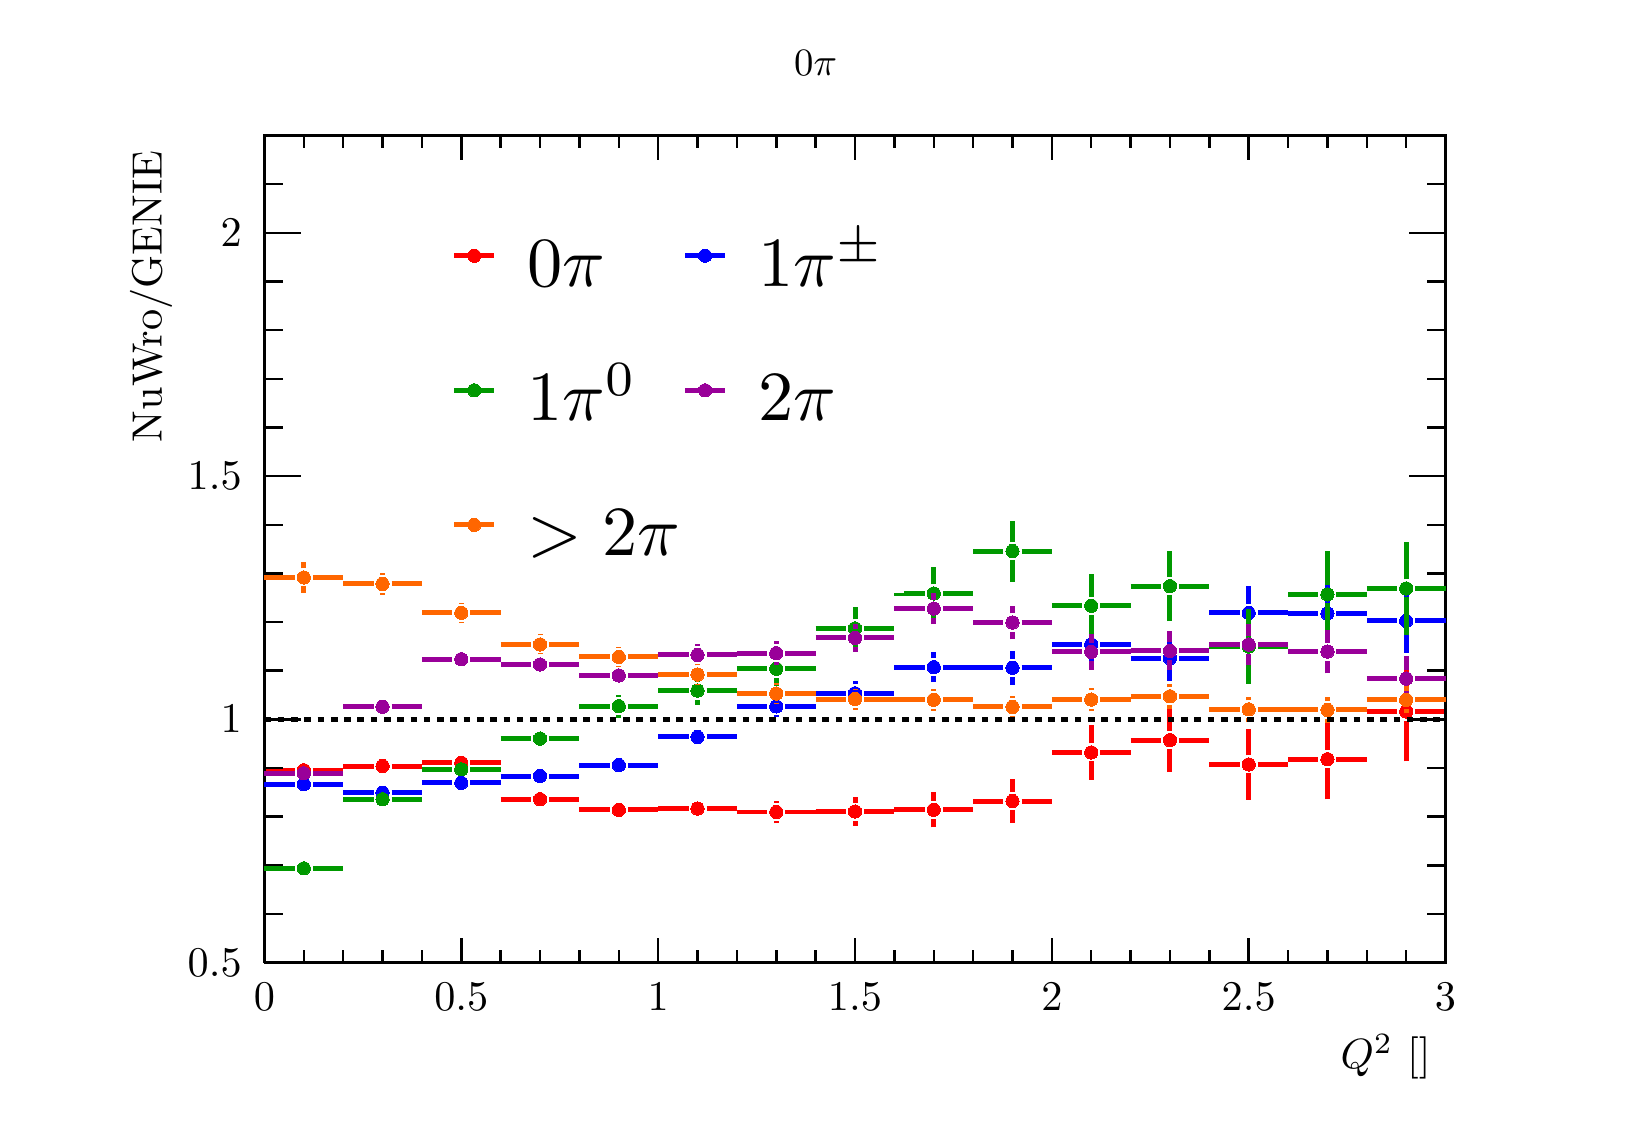
\begin{tikzpicture}
\pgfdeclareplotmark{cross} {
\pgfpathmoveto{\pgfpoint{-0.3\pgfplotmarksize}{\pgfplotmarksize}}
\pgfpathlineto{\pgfpoint{+0.3\pgfplotmarksize}{\pgfplotmarksize}}
\pgfpathlineto{\pgfpoint{+0.3\pgfplotmarksize}{0.3\pgfplotmarksize}}
\pgfpathlineto{\pgfpoint{+1\pgfplotmarksize}{0.3\pgfplotmarksize}}
\pgfpathlineto{\pgfpoint{+1\pgfplotmarksize}{-0.3\pgfplotmarksize}}
\pgfpathlineto{\pgfpoint{+0.3\pgfplotmarksize}{-0.3\pgfplotmarksize}}
\pgfpathlineto{\pgfpoint{+0.3\pgfplotmarksize}{-1.\pgfplotmarksize}}
\pgfpathlineto{\pgfpoint{-0.3\pgfplotmarksize}{-1.\pgfplotmarksize}}
\pgfpathlineto{\pgfpoint{-0.3\pgfplotmarksize}{-0.3\pgfplotmarksize}}
\pgfpathlineto{\pgfpoint{-1.\pgfplotmarksize}{-0.3\pgfplotmarksize}}
\pgfpathlineto{\pgfpoint{-1.\pgfplotmarksize}{0.3\pgfplotmarksize}}
\pgfpathlineto{\pgfpoint{-0.3\pgfplotmarksize}{0.3\pgfplotmarksize}}
\pgfpathclose
\pgfusepathqstroke
}
\pgfdeclareplotmark{cross*} {
\pgfpathmoveto{\pgfpoint{-0.3\pgfplotmarksize}{\pgfplotmarksize}}
\pgfpathlineto{\pgfpoint{+0.3\pgfplotmarksize}{\pgfplotmarksize}}
\pgfpathlineto{\pgfpoint{+0.3\pgfplotmarksize}{0.3\pgfplotmarksize}}
\pgfpathlineto{\pgfpoint{+1\pgfplotmarksize}{0.3\pgfplotmarksize}}
\pgfpathlineto{\pgfpoint{+1\pgfplotmarksize}{-0.3\pgfplotmarksize}}
\pgfpathlineto{\pgfpoint{+0.3\pgfplotmarksize}{-0.3\pgfplotmarksize}}
\pgfpathlineto{\pgfpoint{+0.3\pgfplotmarksize}{-1.\pgfplotmarksize}}
\pgfpathlineto{\pgfpoint{-0.3\pgfplotmarksize}{-1.\pgfplotmarksize}}
\pgfpathlineto{\pgfpoint{-0.3\pgfplotmarksize}{-0.3\pgfplotmarksize}}
\pgfpathlineto{\pgfpoint{-1.\pgfplotmarksize}{-0.3\pgfplotmarksize}}
\pgfpathlineto{\pgfpoint{-1.\pgfplotmarksize}{0.3\pgfplotmarksize}}
\pgfpathlineto{\pgfpoint{-0.3\pgfplotmarksize}{0.3\pgfplotmarksize}}
\pgfpathclose
\pgfusepathqfillstroke
}
\pgfdeclareplotmark{newstar} {
\pgfpathmoveto{\pgfqpoint{0pt}{\pgfplotmarksize}}
\pgfpathlineto{\pgfqpointpolar{44}{0.5\pgfplotmarksize}}
\pgfpathlineto{\pgfqpointpolar{18}{\pgfplotmarksize}}
\pgfpathlineto{\pgfqpointpolar{-20}{0.5\pgfplotmarksize}}
\pgfpathlineto{\pgfqpointpolar{-54}{\pgfplotmarksize}}
\pgfpathlineto{\pgfqpointpolar{-90}{0.5\pgfplotmarksize}}
\pgfpathlineto{\pgfqpointpolar{234}{\pgfplotmarksize}}
\pgfpathlineto{\pgfqpointpolar{198}{0.5\pgfplotmarksize}}
\pgfpathlineto{\pgfqpointpolar{162}{\pgfplotmarksize}}
\pgfpathlineto{\pgfqpointpolar{134}{0.5\pgfplotmarksize}}
\pgfpathclose
\pgfusepathqstroke
}
\pgfdeclareplotmark{newstar*} {
\pgfpathmoveto{\pgfqpoint{0pt}{\pgfplotmarksize}}
\pgfpathlineto{\pgfqpointpolar{44}{0.5\pgfplotmarksize}}
\pgfpathlineto{\pgfqpointpolar{18}{\pgfplotmarksize}}
\pgfpathlineto{\pgfqpointpolar{-20}{0.5\pgfplotmarksize}}
\pgfpathlineto{\pgfqpointpolar{-54}{\pgfplotmarksize}}
\pgfpathlineto{\pgfqpointpolar{-90}{0.5\pgfplotmarksize}}
\pgfpathlineto{\pgfqpointpolar{234}{\pgfplotmarksize}}
\pgfpathlineto{\pgfqpointpolar{198}{0.5\pgfplotmarksize}}
\pgfpathlineto{\pgfqpointpolar{162}{\pgfplotmarksize}}
\pgfpathlineto{\pgfqpointpolar{134}{0.5\pgfplotmarksize}}
\pgfpathclose
\pgfusepathqfillstroke
}
\definecolor{c}{rgb}{1,1,1};
\draw [color=c, fill=c] (0,0) rectangle (20,13.639);
\draw [color=c, fill=c] (3,1.77307) rectangle (18,12.2751);
\definecolor{c}{rgb}{0,0,0};
\draw [c,line width=0.9] (3,1.77307) -- (3,12.2751) -- (18,12.2751) -- (18,1.77307) -- (3,1.77307);
\definecolor{c}{rgb}{1,1,1};
\draw [color=c, fill=c] (3,1.77307) rectangle (18,12.2751);
\definecolor{c}{rgb}{0,0,0};
\draw [c,line width=0.9] (3,1.77307) -- (3,12.2751) -- (18,12.2751) -- (18,1.77307) -- (3,1.77307);
\definecolor{c}{rgb}{1,0,0};
\draw [c,line width=1.8] (3,4.21577) -- (3.38539,4.21577);
\draw [c,line width=1.8] (3.61461,4.21577) -- (4,4.21577);
\foreach \P in {(3.5,4.21577)}{\draw[mark options={color=c,fill=c},mark size=2.402402pt, line width=0.000000pt, mark=*] plot coordinates {\P};}
\draw [c,line width=1.8] (4,4.26895) -- (4.38539,4.26895);
\draw [c,line width=1.8] (4.61461,4.26895) -- (5,4.26895);
\foreach \P in {(4.5,4.26895)}{\draw[mark options={color=c,fill=c},mark size=2.402402pt, line width=0.000000pt, mark=*] plot coordinates {\P};}
\draw [c,line width=1.8] (5,4.31083) -- (5.38539,4.31083);
\draw [c,line width=1.8] (5.61461,4.31083) -- (6,4.31083);
\foreach \P in {(5.5,4.31083)}{\draw[mark options={color=c,fill=c},mark size=2.402402pt, line width=0.000000pt, mark=*] plot coordinates {\P};}
\draw [c,line width=1.8] (6,3.84745) -- (6.38539,3.84745);
\draw [c,line width=1.8] (6.61461,3.84745) -- (7,3.84745);
\foreach \P in {(6.5,3.84745)}{\draw[mark options={color=c,fill=c},mark size=2.402402pt, line width=0.000000pt, mark=*] plot coordinates {\P};}
\draw [c,line width=1.8] (7,3.71127) -- (7.38539,3.71127);
\draw [c,line width=1.8] (7.61461,3.71127) -- (8,3.71127);
\foreach \P in {(7.5,3.71127)}{\draw[mark options={color=c,fill=c},mark size=2.402402pt, line width=0.000000pt, mark=*] plot coordinates {\P};}
\draw [c,line width=1.8] (8,3.72837) -- (8.38539,3.72837);
\draw [c,line width=1.8] (8.61461,3.72837) -- (9,3.72837);
\foreach \P in {(8.5,3.72837)}{\draw[mark options={color=c,fill=c},mark size=2.402402pt, line width=0.000000pt, mark=*] plot coordinates {\P};}
\draw [c,line width=1.8] (9.5,3.54142) -- (9.5,3.57039);
\draw [c,line width=1.8] (9.5,3.79961) -- (9.5,3.82858);
\draw [c,line width=1.8] (9,3.685) -- (9.38539,3.685);
\draw [c,line width=1.8] (9.61461,3.685) -- (10,3.685);
\foreach \P in {(9.5,3.685)}{\draw[mark options={color=c,fill=c},mark size=2.402402pt, line width=0.000000pt, mark=*] plot coordinates {\P};}
\draw [c,line width=1.8] (10.5,3.51081) -- (10.5,3.57643);
\draw [c,line width=1.8] (10.5,3.80565) -- (10.5,3.87127);
\draw [c,line width=1.8] (10,3.69104) -- (10.3854,3.69104);
\draw [c,line width=1.8] (10.6146,3.69104) -- (11,3.69104);
\foreach \P in {(10.5,3.69104)}{\draw[mark options={color=c,fill=c},mark size=2.402402pt, line width=0.000000pt, mark=*] plot coordinates {\P};}
\draw [c,line width=1.8] (11.5,3.49068) -- (11.5,3.59871);
\draw [c,line width=1.8] (11.5,3.82794) -- (11.5,3.93597);
\draw [c,line width=1.8] (11,3.71333) -- (11.3854,3.71333);
\draw [c,line width=1.8] (11.6146,3.71333) -- (12,3.71333);
\foreach \P in {(11.5,3.71333)}{\draw[mark options={color=c,fill=c},mark size=2.402402pt, line width=0.000000pt, mark=*] plot coordinates {\P};}
\draw [c,line width=1.8] (12.5,3.54863) -- (12.5,3.70938);
\draw [c,line width=1.8] (12.5,3.9386) -- (12.5,4.09935);
\draw [c,line width=1.8] (12,3.82399) -- (12.3854,3.82399);
\draw [c,line width=1.8] (12.6146,3.82399) -- (13,3.82399);
\foreach \P in {(12.5,3.82399)}{\draw[mark options={color=c,fill=c},mark size=2.402402pt, line width=0.000000pt, mark=*] plot coordinates {\P};}
\draw [c,line width=1.8] (13.5,4.09501) -- (13.5,4.32686);
\draw [c,line width=1.8] (13.5,4.55609) -- (13.5,4.78794);
\draw [c,line width=1.8] (13,4.44148) -- (13.3854,4.44148);
\draw [c,line width=1.8] (13.6146,4.44148) -- (14,4.44148);
\foreach \P in {(13.5,4.44148)}{\draw[mark options={color=c,fill=c},mark size=2.402402pt, line width=0.000000pt, mark=*] plot coordinates {\P};}
\draw [c,line width=1.8] (14.5,4.19047) -- (14.5,4.48288);
\draw [c,line width=1.8] (14.5,4.71211) -- (14.5,5.00453);
\draw [c,line width=1.8] (14,4.5975) -- (14.3854,4.5975);
\draw [c,line width=1.8] (14.6146,4.5975) -- (15,4.5975);
\foreach \P in {(14.5,4.5975)}{\draw[mark options={color=c,fill=c},mark size=2.402402pt, line width=0.000000pt, mark=*] plot coordinates {\P};}
\draw [c,line width=1.8] (15.5,3.83985) -- (15.5,4.1741);
\draw [c,line width=1.8] (15.5,4.40333) -- (15.5,4.73759);
\draw [c,line width=1.8] (15,4.28872) -- (15.3854,4.28872);
\draw [c,line width=1.8] (15.6146,4.28872) -- (16,4.28872);
\foreach \P in {(15.5,4.28872)}{\draw[mark options={color=c,fill=c},mark size=2.402402pt, line width=0.000000pt, mark=*] plot coordinates {\P};}
\draw [c,line width=1.8] (16.5,3.84563) -- (16.5,4.24124);
\draw [c,line width=1.8] (16.5,4.47047) -- (16.5,4.86609);
\draw [c,line width=1.8] (16,4.35586) -- (16.3854,4.35586);
\draw [c,line width=1.8] (16.6146,4.35586) -- (17,4.35586);
\foreach \P in {(16.5,4.35586)}{\draw[mark options={color=c,fill=c},mark size=2.402402pt, line width=0.000000pt, mark=*] plot coordinates {\P};}
\draw [c,line width=1.8] (17.5,4.32693) -- (17.5,4.84686);
\draw [c,line width=1.8] (17.5,5.07609) -- (17.5,5.59602);
\draw [c,line width=1.8] (17,4.96148) -- (17.3854,4.96148);
\draw [c,line width=1.8] (17.6146,4.96148) -- (18,4.96148);
\foreach \P in {(17.5,4.96148)}{\draw[mark options={color=c,fill=c},mark size=2.402402pt, line width=0.000000pt, mark=*] plot coordinates {\P};}
\definecolor{c}{rgb}{0,0,0};
\draw [c,line width=0.9] (3,1.77307) -- (18,1.77307);
\draw [c,line width=0.9] (3,2.07994) -- (3,1.77307);
\draw [c,line width=0.9] (3.5,1.9265) -- (3.5,1.77307);
\draw [c,line width=0.9] (4,1.9265) -- (4,1.77307);
\draw [c,line width=0.9] (4.5,1.9265) -- (4.5,1.77307);
\draw [c,line width=0.9] (5,1.9265) -- (5,1.77307);
\draw [c,line width=0.9] (5.5,2.07994) -- (5.5,1.77307);
\draw [c,line width=0.9] (6,1.9265) -- (6,1.77307);
\draw [c,line width=0.9] (6.5,1.9265) -- (6.5,1.77307);
\draw [c,line width=0.9] (7,1.9265) -- (7,1.77307);
\draw [c,line width=0.9] (7.5,1.9265) -- (7.5,1.77307);
\draw [c,line width=0.9] (8,2.07994) -- (8,1.77307);
\draw [c,line width=0.9] (8.5,1.9265) -- (8.5,1.77307);
\draw [c,line width=0.9] (9,1.9265) -- (9,1.77307);
\draw [c,line width=0.9] (9.5,1.9265) -- (9.5,1.77307);
\draw [c,line width=0.9] (10,1.9265) -- (10,1.77307);
\draw [c,line width=0.9] (10.5,2.07994) -- (10.5,1.77307);
\draw [c,line width=0.9] (11,1.9265) -- (11,1.77307);
\draw [c,line width=0.9] (11.5,1.9265) -- (11.5,1.77307);
\draw [c,line width=0.9] (12,1.9265) -- (12,1.77307);
\draw [c,line width=0.9] (12.5,1.9265) -- (12.5,1.77307);
\draw [c,line width=0.9] (13,2.07994) -- (13,1.77307);
\draw [c,line width=0.9] (13.5,1.9265) -- (13.5,1.77307);
\draw [c,line width=0.9] (14,1.9265) -- (14,1.77307);
\draw [c,line width=0.9] (14.5,1.9265) -- (14.5,1.77307);
\draw [c,line width=0.9] (15,1.9265) -- (15,1.77307);
\draw [c,line width=0.9] (15.5,2.07994) -- (15.5,1.77307);
\draw [c,line width=0.9] (16,1.9265) -- (16,1.77307);
\draw [c,line width=0.9] (16.5,1.9265) -- (16.5,1.77307);
\draw [c,line width=0.9] (17,1.9265) -- (17,1.77307);
\draw [c,line width=0.9] (17.5,1.9265) -- (17.5,1.77307);
\draw [c,line width=0.9] (18,2.07994) -- (18,1.77307);
\draw [c,line width=0.9] (18,2.07994) -- (18,1.77307);
\draw [anchor=base] (3,1.15931) node[scale=1.52731, color=c, rotate=0]{0};
\draw [anchor=base] (5.5,1.15931) node[scale=1.52731, color=c, rotate=0]{0.5};
\draw [anchor=base] (8,1.15931) node[scale=1.52731, color=c, rotate=0]{1};
\draw [anchor=base] (10.5,1.15931) node[scale=1.52731, color=c, rotate=0]{1.5};
\draw [anchor=base] (13,1.15931) node[scale=1.52731, color=c, rotate=0]{2};
\draw [anchor=base] (15.5,1.15931) node[scale=1.52731, color=c, rotate=0]{2.5};
\draw [anchor=base] (18,1.15931) node[scale=1.52731, color=c, rotate=0]{3};
\draw [anchor= east] (18,0.572837) node[scale=1.52731, color=c, rotate=0]{$Q^{2}$ [\si{\GeV\squared}] };
\draw [c,line width=0.9] (3,12.2751) -- (18,12.2751);
\draw [c,line width=0.9] (3,11.9682) -- (3,12.2751);
\draw [c,line width=0.9] (3.5,12.1216) -- (3.5,12.2751);
\draw [c,line width=0.9] (4,12.1216) -- (4,12.2751);
\draw [c,line width=0.9] (4.5,12.1216) -- (4.5,12.2751);
\draw [c,line width=0.9] (5,12.1216) -- (5,12.2751);
\draw [c,line width=0.9] (5.5,11.9682) -- (5.5,12.2751);
\draw [c,line width=0.9] (6,12.1216) -- (6,12.2751);
\draw [c,line width=0.9] (6.5,12.1216) -- (6.5,12.2751);
\draw [c,line width=0.9] (7,12.1216) -- (7,12.2751);
\draw [c,line width=0.9] (7.5,12.1216) -- (7.5,12.2751);
\draw [c,line width=0.9] (8,11.9682) -- (8,12.2751);
\draw [c,line width=0.9] (8.5,12.1216) -- (8.5,12.2751);
\draw [c,line width=0.9] (9,12.1216) -- (9,12.2751);
\draw [c,line width=0.9] (9.5,12.1216) -- (9.5,12.2751);
\draw [c,line width=0.9] (10,12.1216) -- (10,12.2751);
\draw [c,line width=0.9] (10.5,11.9682) -- (10.5,12.2751);
\draw [c,line width=0.9] (11,12.1216) -- (11,12.2751);
\draw [c,line width=0.9] (11.5,12.1216) -- (11.5,12.2751);
\draw [c,line width=0.9] (12,12.1216) -- (12,12.2751);
\draw [c,line width=0.9] (12.5,12.1216) -- (12.5,12.2751);
\draw [c,line width=0.9] (13,11.9682) -- (13,12.2751);
\draw [c,line width=0.9] (13.5,12.1216) -- (13.5,12.2751);
\draw [c,line width=0.9] (14,12.1216) -- (14,12.2751);
\draw [c,line width=0.9] (14.5,12.1216) -- (14.5,12.2751);
\draw [c,line width=0.9] (15,12.1216) -- (15,12.2751);
\draw [c,line width=0.9] (15.5,11.9682) -- (15.5,12.2751);
\draw [c,line width=0.9] (16,12.1216) -- (16,12.2751);
\draw [c,line width=0.9] (16.5,12.1216) -- (16.5,12.2751);
\draw [c,line width=0.9] (17,12.1216) -- (17,12.2751);
\draw [c,line width=0.9] (17.5,12.1216) -- (17.5,12.2751);
\draw [c,line width=0.9] (18,11.9682) -- (18,12.2751);
\draw [c,line width=0.9] (18,11.9682) -- (18,12.2751);
\draw [c,line width=0.9] (3,1.77307) -- (3,12.2751);
\draw [c,line width=0.9] (3.462,1.77307) -- (3,1.77307);
\draw [c,line width=0.9] (3.231,2.39083) -- (3,2.39083);
\draw [c,line width=0.9] (3.231,3.0086) -- (3,3.0086);
\draw [c,line width=0.9] (3.231,3.62636) -- (3,3.62636);
\draw [c,line width=0.9] (3.231,4.24413) -- (3,4.24413);
\draw [c,line width=0.9] (3.462,4.86189) -- (3,4.86189);
\draw [c,line width=0.9] (3.231,5.47966) -- (3,5.47966);
\draw [c,line width=0.9] (3.231,6.09742) -- (3,6.09742);
\draw [c,line width=0.9] (3.231,6.71519) -- (3,6.71519);
\draw [c,line width=0.9] (3.231,7.33295) -- (3,7.33295);
\draw [c,line width=0.9] (3.462,7.95072) -- (3,7.95072);
\draw [c,line width=0.9] (3.231,8.56848) -- (3,8.56848);
\draw [c,line width=0.9] (3.231,9.18625) -- (3,9.18625);
\draw [c,line width=0.9] (3.231,9.80401) -- (3,9.80401);
\draw [c,line width=0.9] (3.231,10.4218) -- (3,10.4218);
\draw [c,line width=0.9] (3.462,11.0395) -- (3,11.0395);
\draw [c,line width=0.9] (3.462,11.0395) -- (3,11.0395);
\draw [c,line width=0.9] (3.231,11.6573) -- (3,11.6573);
\draw [c,line width=0.9] (3.231,12.2751) -- (3,12.2751);
\draw [anchor= east] (2.9,1.77307) node[scale=1.52731, color=c, rotate=0]{0.5};
\draw [anchor= east] (2.9,4.86189) node[scale=1.52731, color=c, rotate=0]{1};
\draw [anchor= east] (2.9,7.95072) node[scale=1.52731, color=c, rotate=0]{1.5};
\draw [anchor= east] (2.9,11.0395) node[scale=1.52731, color=c, rotate=0]{2};
\draw [anchor= east] (1.56,12.2751) node[scale=1.52731, color=c, rotate=90]{ NuWro/GENIE};
\draw [c,line width=0.9] (18,1.77307) -- (18,12.2751);
\draw [c,line width=0.9] (17.538,1.77307) -- (18,1.77307);
\draw [c,line width=0.9] (17.769,2.39083) -- (18,2.39083);
\draw [c,line width=0.9] (17.769,3.0086) -- (18,3.0086);
\draw [c,line width=0.9] (17.769,3.62636) -- (18,3.62636);
\draw [c,line width=0.9] (17.769,4.24413) -- (18,4.24413);
\draw [c,line width=0.9] (17.538,4.86189) -- (18,4.86189);
\draw [c,line width=0.9] (17.769,5.47966) -- (18,5.47966);
\draw [c,line width=0.9] (17.769,6.09742) -- (18,6.09742);
\draw [c,line width=0.9] (17.769,6.71519) -- (18,6.71519);
\draw [c,line width=0.9] (17.769,7.33295) -- (18,7.33295);
\draw [c,line width=0.9] (17.538,7.95072) -- (18,7.95072);
\draw [c,line width=0.9] (17.769,8.56848) -- (18,8.56848);
\draw [c,line width=0.9] (17.769,9.18625) -- (18,9.18625);
\draw [c,line width=0.9] (17.769,9.80401) -- (18,9.80401);
\draw [c,line width=0.9] (17.769,10.4218) -- (18,10.4218);
\draw [c,line width=0.9] (17.538,11.0395) -- (18,11.0395);
\draw [c,line width=0.9] (17.538,11.0395) -- (18,11.0395);
\draw [c,line width=0.9] (17.769,11.6573) -- (18,11.6573);
\draw [c,line width=0.9] (17.769,12.2751) -- (18,12.2751);
\definecolor{c}{rgb}{0,0,1};
\draw [c,line width=1.8] (3,4.03842) -- (3.38539,4.03842);
\draw [c,line width=1.8] (3.61461,4.03842) -- (4,4.03842);
\foreach \P in {(3.5,4.03842)}{\draw[mark options={color=c,fill=c},mark size=2.402402pt, line width=0.000000pt, mark=*] plot coordinates {\P};}
\draw [c,line width=1.8] (4,3.92971) -- (4.38539,3.92971);
\draw [c,line width=1.8] (4.61461,3.92971) -- (5,3.92971);
\foreach \P in {(4.5,3.92971)}{\draw[mark options={color=c,fill=c},mark size=2.402402pt, line width=0.000000pt, mark=*] plot coordinates {\P};}
\draw [c,line width=1.8] (5,4.05491) -- (5.38539,4.05491);
\draw [c,line width=1.8] (5.61461,4.05491) -- (6,4.05491);
\foreach \P in {(5.5,4.05491)}{\draw[mark options={color=c,fill=c},mark size=2.402402pt, line width=0.000000pt, mark=*] plot coordinates {\P};}
\draw [c,line width=1.8] (6,4.14205) -- (6.38539,4.14205);
\draw [c,line width=1.8] (6.61461,4.14205) -- (7,4.14205);
\foreach \P in {(6.5,4.14205)}{\draw[mark options={color=c,fill=c},mark size=2.402402pt, line width=0.000000pt, mark=*] plot coordinates {\P};}
\draw [c,line width=1.8] (7,4.28102) -- (7.38539,4.28102);
\draw [c,line width=1.8] (7.61461,4.28102) -- (8,4.28102);
\foreach \P in {(7.5,4.28102)}{\draw[mark options={color=c,fill=c},mark size=2.402402pt, line width=0.000000pt, mark=*] plot coordinates {\P};}
\draw [c,line width=1.8] (8,4.63816) -- (8.38539,4.63816);
\draw [c,line width=1.8] (8.61461,4.63816) -- (9,4.63816);
\foreach \P in {(8.5,4.63816)}{\draw[mark options={color=c,fill=c},mark size=2.402402pt, line width=0.000000pt, mark=*] plot coordinates {\P};}
\draw [c,line width=1.8] (9.5,4.89659) -- (9.5,4.91156);
\draw [c,line width=1.8] (9.5,5.14079) -- (9.5,5.15576);
\draw [c,line width=1.8] (9,5.02618) -- (9.38539,5.02618);
\draw [c,line width=1.8] (9.61461,5.02618) -- (10,5.02618);
\foreach \P in {(9.5,5.02618)}{\draw[mark options={color=c,fill=c},mark size=2.402402pt, line width=0.000000pt, mark=*] plot coordinates {\P};}
\draw [c,line width=1.8] (10.5,5.03532) -- (10.5,5.07793);
\draw [c,line width=1.8] (10.5,5.30715) -- (10.5,5.34976);
\draw [c,line width=1.8] (10,5.19254) -- (10.3854,5.19254);
\draw [c,line width=1.8] (10.6146,5.19254) -- (11,5.19254);
\foreach \P in {(10.5,5.19254)}{\draw[mark options={color=c,fill=c},mark size=2.402402pt, line width=0.000000pt, mark=*] plot coordinates {\P};}
\draw [c,line width=1.8] (11.5,5.3355) -- (11.5,5.41019);
\draw [c,line width=1.8] (11.5,5.63942) -- (11.5,5.71411);
\draw [c,line width=1.8] (11,5.5248) -- (11.3854,5.5248);
\draw [c,line width=1.8] (11.6146,5.5248) -- (12,5.5248);
\foreach \P in {(11.5,5.5248)}{\draw[mark options={color=c,fill=c},mark size=2.402402pt, line width=0.000000pt, mark=*] plot coordinates {\P};}
\draw [c,line width=1.8] (12.5,5.29966) -- (12.5,5.40154);
\draw [c,line width=1.8] (12.5,5.63077) -- (12.5,5.73265);
\draw [c,line width=1.8] (12,5.51616) -- (12.3854,5.51616);
\draw [c,line width=1.8] (12.6146,5.51616) -- (13,5.51616);
\foreach \P in {(12.5,5.51616)}{\draw[mark options={color=c,fill=c},mark size=2.402402pt, line width=0.000000pt, mark=*] plot coordinates {\P};}
\draw [c,line width=1.8] (13.5,5.55623) -- (13.5,5.6978);
\draw [c,line width=1.8] (13.5,5.92703) -- (13.5,6.06861);
\draw [c,line width=1.8] (13,5.81242) -- (13.3854,5.81242);
\draw [c,line width=1.8] (13.6146,5.81242) -- (14,5.81242);
\foreach \P in {(13.5,5.81242)}{\draw[mark options={color=c,fill=c},mark size=2.402402pt, line width=0.000000pt, mark=*] plot coordinates {\P};}
\draw [c,line width=1.8] (14.5,5.35062) -- (14.5,5.52348);
\draw [c,line width=1.8] (14.5,5.75271) -- (14.5,5.92556);
\draw [c,line width=1.8] (14,5.63809) -- (14.3854,5.63809);
\draw [c,line width=1.8] (14.6146,5.63809) -- (15,5.63809);
\foreach \P in {(14.5,5.63809)}{\draw[mark options={color=c,fill=c},mark size=2.402402pt, line width=0.000000pt, mark=*] plot coordinates {\P};}
\draw [c,line width=1.8] (15.5,5.87644) -- (15.5,6.09821);
\draw [c,line width=1.8] (15.5,6.32743) -- (15.5,6.5492);
\draw [c,line width=1.8] (15,6.21282) -- (15.3854,6.21282);
\draw [c,line width=1.8] (15.6146,6.21282) -- (16,6.21282);
\foreach \P in {(15.5,6.21282)}{\draw[mark options={color=c,fill=c},mark size=2.402402pt, line width=0.000000pt, mark=*] plot coordinates {\P};}
\draw [c,line width=1.8] (16.5,5.8388) -- (16.5,6.09164);
\draw [c,line width=1.8] (16.5,6.32087) -- (16.5,6.5737);
\draw [c,line width=1.8] (16,6.20625) -- (16.3854,6.20625);
\draw [c,line width=1.8] (16.6146,6.20625) -- (17,6.20625);
\foreach \P in {(16.5,6.20625)}{\draw[mark options={color=c,fill=c},mark size=2.402402pt, line width=0.000000pt, mark=*] plot coordinates {\P};}
\draw [c,line width=1.8] (17.5,5.71038) -- (17.5,5.99691);
\draw [c,line width=1.8] (17.5,6.22613) -- (17.5,6.51266);
\draw [c,line width=1.8] (17,6.11152) -- (17.3854,6.11152);
\draw [c,line width=1.8] (17.6146,6.11152) -- (18,6.11152);
\foreach \P in {(17.5,6.11152)}{\draw[mark options={color=c,fill=c},mark size=2.402402pt, line width=0.000000pt, mark=*] plot coordinates {\P};}
\definecolor{c}{rgb}{0,0.6,0};
\draw [c,line width=1.8] (3,2.96963) -- (3.38539,2.96963);
\draw [c,line width=1.8] (3.61461,2.96963) -- (4,2.96963);
\foreach \P in {(3.5,2.96963)}{\draw[mark options={color=c,fill=c},mark size=2.402402pt, line width=0.000000pt, mark=*] plot coordinates {\P};}
\draw [c,line width=1.8] (4,3.84623) -- (4.38539,3.84623);
\draw [c,line width=1.8] (4.61461,3.84623) -- (5,3.84623);
\foreach \P in {(4.5,3.84623)}{\draw[mark options={color=c,fill=c},mark size=2.402402pt, line width=0.000000pt, mark=*] plot coordinates {\P};}
\draw [c,line width=1.8] (5,4.22718) -- (5.38539,4.22718);
\draw [c,line width=1.8] (5.61461,4.22718) -- (6,4.22718);
\foreach \P in {(5.5,4.22718)}{\draw[mark options={color=c,fill=c},mark size=2.402402pt, line width=0.000000pt, mark=*] plot coordinates {\P};}
\draw [c,line width=1.8] (6,4.61757) -- (6.38539,4.61757);
\draw [c,line width=1.8] (6.61461,4.61757) -- (7,4.61757);
\foreach \P in {(6.5,4.61757)}{\draw[mark options={color=c,fill=c},mark size=2.402402pt, line width=0.000000pt, mark=*] plot coordinates {\P};}
\draw [c,line width=1.8] (7.5,4.88296) -- (7.5,4.91453);
\draw [c,line width=1.8] (7.5,5.14375) -- (7.5,5.17532);
\draw [c,line width=1.8] (7,5.02914) -- (7.38539,5.02914);
\draw [c,line width=1.8] (7.61461,5.02914) -- (8,5.02914);
\foreach \P in {(7.5,5.02914)}{\draw[mark options={color=c,fill=c},mark size=2.402402pt, line width=0.000000pt, mark=*] plot coordinates {\P};}
\draw [c,line width=1.8] (8.5,5.04595) -- (8.5,5.11186);
\draw [c,line width=1.8] (8.5,5.34109) -- (8.5,5.407);
\draw [c,line width=1.8] (8,5.22648) -- (8.38539,5.22648);
\draw [c,line width=1.8] (8.61461,5.22648) -- (9,5.22648);
\foreach \P in {(8.5,5.22648)}{\draw[mark options={color=c,fill=c},mark size=2.402402pt, line width=0.000000pt, mark=*] plot coordinates {\P};}
\draw [c,line width=1.8] (9.5,5.28296) -- (9.5,5.38934);
\draw [c,line width=1.8] (9.5,5.61857) -- (9.5,5.72495);
\draw [c,line width=1.8] (9,5.50395) -- (9.38539,5.50395);
\draw [c,line width=1.8] (9.61461,5.50395) -- (10,5.50395);
\foreach \P in {(9.5,5.50395)}{\draw[mark options={color=c,fill=c},mark size=2.402402pt, line width=0.000000pt, mark=*] plot coordinates {\P};}
\draw [c,line width=1.8] (10.5,5.74173) -- (10.5,5.90201);
\draw [c,line width=1.8] (10.5,6.13123) -- (10.5,6.29151);
\draw [c,line width=1.8] (10,6.01662) -- (10.3854,6.01662);
\draw [c,line width=1.8] (10.6146,6.01662) -- (11,6.01662);
\foreach \P in {(10.5,6.01662)}{\draw[mark options={color=c,fill=c},mark size=2.402402pt, line width=0.000000pt, mark=*] plot coordinates {\P};}
\draw [c,line width=1.8] (11.5,6.13014) -- (11.5,6.34595);
\draw [c,line width=1.8] (11.5,6.57518) -- (11.5,6.79099);
\draw [c,line width=1.8] (11,6.46056) -- (11.3854,6.46056);
\draw [c,line width=1.8] (11.6146,6.46056) -- (12,6.46056);
\foreach \P in {(11.5,6.46056)}{\draw[mark options={color=c,fill=c},mark size=2.402402pt, line width=0.000000pt, mark=*] plot coordinates {\P};}
\draw [c,line width=1.8] (12.5,6.61102) -- (12.5,6.88403);
\draw [c,line width=1.8] (12.5,7.11326) -- (12.5,7.38627);
\draw [c,line width=1.8] (12,6.99864) -- (12.3854,6.99864);
\draw [c,line width=1.8] (12.6146,6.99864) -- (13,6.99864);
\foreach \P in {(12.5,6.99864)}{\draw[mark options={color=c,fill=c},mark size=2.402402pt, line width=0.000000pt, mark=*] plot coordinates {\P};}
\draw [c,line width=1.8] (13.5,5.89746) -- (13.5,6.18967);
\draw [c,line width=1.8] (13.5,6.4189) -- (13.5,6.71111);
\draw [c,line width=1.8] (13,6.30429) -- (13.3854,6.30429);
\draw [c,line width=1.8] (13.6146,6.30429) -- (14,6.30429);
\foreach \P in {(13.5,6.30429)}{\draw[mark options={color=c,fill=c},mark size=2.402402pt, line width=0.000000pt, mark=*] plot coordinates {\P};}
\draw [c,line width=1.8] (14.5,6.10887) -- (14.5,6.4385);
\draw [c,line width=1.8] (14.5,6.66772) -- (14.5,6.99735);
\draw [c,line width=1.8] (14,6.55311) -- (14.3854,6.55311);
\draw [c,line width=1.8] (14.6146,6.55311) -- (15,6.55311);
\foreach \P in {(14.5,6.55311)}{\draw[mark options={color=c,fill=c},mark size=2.402402pt, line width=0.000000pt, mark=*] plot coordinates {\P};}
\draw [c,line width=1.8] (15.5,5.31219) -- (15.5,5.67124);
\draw [c,line width=1.8] (15.5,5.90047) -- (15.5,6.25952);
\draw [c,line width=1.8] (15,5.78585) -- (15.3854,5.78585);
\draw [c,line width=1.8] (15.6146,5.78585) -- (16,5.78585);
\foreach \P in {(15.5,5.78585)}{\draw[mark options={color=c,fill=c},mark size=2.402402pt, line width=0.000000pt, mark=*] plot coordinates {\P};}
\draw [c,line width=1.8] (16.5,5.89275) -- (16.5,6.33367);
\draw [c,line width=1.8] (16.5,6.56289) -- (16.5,7.00381);
\draw [c,line width=1.8] (16,6.44828) -- (16.3854,6.44828);
\draw [c,line width=1.8] (16.6146,6.44828) -- (17,6.44828);
\foreach \P in {(16.5,6.44828)}{\draw[mark options={color=c,fill=c},mark size=2.402402pt, line width=0.000000pt, mark=*] plot coordinates {\P};}
\draw [c,line width=1.8] (17.5,5.93881) -- (17.5,6.40983);
\draw [c,line width=1.8] (17.5,6.63906) -- (17.5,7.11009);
\draw [c,line width=1.8] (17,6.52445) -- (17.3854,6.52445);
\draw [c,line width=1.8] (17.6146,6.52445) -- (18,6.52445);
\foreach \P in {(17.5,6.52445)}{\draw[mark options={color=c,fill=c},mark size=2.402402pt, line width=0.000000pt, mark=*] plot coordinates {\P};}
\definecolor{c}{rgb}{0.6,0,0.6};
\draw [c,line width=1.8] (3,4.17734) -- (3.38539,4.17734);
\draw [c,line width=1.8] (3.61461,4.17734) -- (4,4.17734);
\foreach \P in {(3.5,4.17734)}{\draw[mark options={color=c,fill=c},mark size=2.402402pt, line width=0.000000pt, mark=*] plot coordinates {\P};}
\draw [c,line width=1.8] (4,5.02168) -- (4.38539,5.02168);
\draw [c,line width=1.8] (4.61461,5.02168) -- (5,5.02168);
\foreach \P in {(4.5,5.02168)}{\draw[mark options={color=c,fill=c},mark size=2.402402pt, line width=0.000000pt, mark=*] plot coordinates {\P};}
\draw [c,line width=1.8] (5,5.62536) -- (5.38539,5.62536);
\draw [c,line width=1.8] (5.61461,5.62536) -- (6,5.62536);
\foreach \P in {(5.5,5.62536)}{\draw[mark options={color=c,fill=c},mark size=2.402402pt, line width=0.000000pt, mark=*] plot coordinates {\P};}
\draw [c,line width=1.8] (6,5.55861) -- (6.38539,5.55861);
\draw [c,line width=1.8] (6.61461,5.55861) -- (7,5.55861);
\foreach \P in {(6.5,5.55861)}{\draw[mark options={color=c,fill=c},mark size=2.402402pt, line width=0.000000pt, mark=*] plot coordinates {\P};}
\draw [c,line width=1.8] (7,5.41943) -- (7.38539,5.41943);
\draw [c,line width=1.8] (7.61461,5.41943) -- (8,5.41943);
\foreach \P in {(7.5,5.41943)}{\draw[mark options={color=c,fill=c},mark size=2.402402pt, line width=0.000000pt, mark=*] plot coordinates {\P};}
\draw [c,line width=1.8] (8.5,5.54664) -- (8.5,5.56522);
\draw [c,line width=1.8] (8.5,5.79444) -- (8.5,5.81302);
\draw [c,line width=1.8] (8,5.67983) -- (8.38539,5.67983);
\draw [c,line width=1.8] (8.61461,5.67983) -- (9,5.67983);
\foreach \P in {(8.5,5.67983)}{\draw[mark options={color=c,fill=c},mark size=2.402402pt, line width=0.000000pt, mark=*] plot coordinates {\P};}
\draw [c,line width=1.8] (9.5,5.55105) -- (9.5,5.5874);
\draw [c,line width=1.8] (9.5,5.81663) -- (9.5,5.85297);
\draw [c,line width=1.8] (9,5.70201) -- (9.38539,5.70201);
\draw [c,line width=1.8] (9.61461,5.70201) -- (10,5.70201);
\foreach \P in {(9.5,5.70201)}{\draw[mark options={color=c,fill=c},mark size=2.402402pt, line width=0.000000pt, mark=*] plot coordinates {\P};}
\draw [c,line width=1.8] (10.5,5.72206) -- (10.5,5.78243);
\draw [c,line width=1.8] (10.5,6.01165) -- (10.5,6.07202);
\draw [c,line width=1.8] (10,5.89704) -- (10.3854,5.89704);
\draw [c,line width=1.8] (10.6146,5.89704) -- (11,5.89704);
\foreach \P in {(10.5,5.89704)}{\draw[mark options={color=c,fill=c},mark size=2.402402pt, line width=0.000000pt, mark=*] plot coordinates {\P};}
\draw [c,line width=1.8] (11.5,6.07114) -- (11.5,6.15359);
\draw [c,line width=1.8] (11.5,6.38282) -- (11.5,6.46527);
\draw [c,line width=1.8] (11,6.2682) -- (11.3854,6.2682);
\draw [c,line width=1.8] (11.6146,6.2682) -- (12,6.2682);
\foreach \P in {(11.5,6.2682)}{\draw[mark options={color=c,fill=c},mark size=2.402402pt, line width=0.000000pt, mark=*] plot coordinates {\P};}
\draw [c,line width=1.8] (12.5,5.87766) -- (12.5,5.97701);
\draw [c,line width=1.8] (12.5,6.20624) -- (12.5,6.30558);
\draw [c,line width=1.8] (12,6.09162) -- (12.3854,6.09162);
\draw [c,line width=1.8] (12.6146,6.09162) -- (13,6.09162);
\foreach \P in {(12.5,6.09162)}{\draw[mark options={color=c,fill=c},mark size=2.402402pt, line width=0.000000pt, mark=*] plot coordinates {\P};}
\draw [c,line width=1.8] (13.5,5.49448) -- (13.5,5.60402);
\draw [c,line width=1.8] (13.5,5.83325) -- (13.5,5.94279);
\draw [c,line width=1.8] (13,5.71863) -- (13.3854,5.71863);
\draw [c,line width=1.8] (13.6146,5.71863) -- (14,5.71863);
\foreach \P in {(13.5,5.71863)}{\draw[mark options={color=c,fill=c},mark size=2.402402pt, line width=0.000000pt, mark=*] plot coordinates {\P};}
\draw [c,line width=1.8] (14.5,5.48628) -- (14.5,5.61738);
\draw [c,line width=1.8] (14.5,5.8466) -- (14.5,5.97771);
\draw [c,line width=1.8] (14,5.73199) -- (14.3854,5.73199);
\draw [c,line width=1.8] (14.6146,5.73199) -- (15,5.73199);
\foreach \P in {(14.5,5.73199)}{\draw[mark options={color=c,fill=c},mark size=2.402402pt, line width=0.000000pt, mark=*] plot coordinates {\P};}
\draw [c,line width=1.8] (15.5,5.5459) -- (15.5,5.69685);
\draw [c,line width=1.8] (15.5,5.92608) -- (15.5,6.07703);
\draw [c,line width=1.8] (15,5.81147) -- (15.3854,5.81147);
\draw [c,line width=1.8] (15.6146,5.81147) -- (16,5.81147);
\foreach \P in {(15.5,5.81147)}{\draw[mark options={color=c,fill=c},mark size=2.402402pt, line width=0.000000pt, mark=*] plot coordinates {\P};}
\draw [c,line width=1.8] (16.5,5.44455) -- (16.5,5.60772);
\draw [c,line width=1.8] (16.5,5.83695) -- (16.5,6.00011);
\draw [c,line width=1.8] (16,5.72233) -- (16.3854,5.72233);
\draw [c,line width=1.8] (16.6146,5.72233) -- (17,5.72233);
\foreach \P in {(16.5,5.72233)}{\draw[mark options={color=c,fill=c},mark size=2.402402pt, line width=0.000000pt, mark=*] plot coordinates {\P};}
\draw [c,line width=1.8] (17.5,5.09002) -- (17.5,5.26421);
\draw [c,line width=1.8] (17.5,5.49344) -- (17.5,5.66763);
\draw [c,line width=1.8] (17,5.37883) -- (17.3854,5.37883);
\draw [c,line width=1.8] (17.6146,5.37883) -- (18,5.37883);
\foreach \P in {(17.5,5.37883)}{\draw[mark options={color=c,fill=c},mark size=2.402402pt, line width=0.000000pt, mark=*] plot coordinates {\P};}
\definecolor{c}{rgb}{1,0.4,0};
\draw [c,line width=1.8] (3.5,6.46761) -- (3.5,6.54886);
\draw [c,line width=1.8] (3.5,6.77809) -- (3.5,6.85934);
\draw [c,line width=1.8] (3,6.66348) -- (3.38539,6.66348);
\draw [c,line width=1.8] (3.61461,6.66348) -- (4,6.66348);
\foreach \P in {(3.5,6.66348)}{\draw[mark options={color=c,fill=c},mark size=2.402402pt, line width=0.000000pt, mark=*] plot coordinates {\P};}
\draw [c,line width=1.8] (4.5,6.44341) -- (4.5,6.46763);
\draw [c,line width=1.8] (4.5,6.69685) -- (4.5,6.72107);
\draw [c,line width=1.8] (4,6.58224) -- (4.38539,6.58224);
\draw [c,line width=1.8] (4.61461,6.58224) -- (5,6.58224);
\foreach \P in {(4.5,6.58224)}{\draw[mark options={color=c,fill=c},mark size=2.402402pt, line width=0.000000pt, mark=*] plot coordinates {\P};}
\draw [c,line width=1.8] (5.5,6.08483) -- (5.5,6.10007);
\draw [c,line width=1.8] (5.5,6.3293) -- (5.5,6.34454);
\draw [c,line width=1.8] (5,6.21468) -- (5.38539,6.21468);
\draw [c,line width=1.8] (5.61461,6.21468) -- (6,6.21468);
\foreach \P in {(5.5,6.21468)}{\draw[mark options={color=c,fill=c},mark size=2.402402pt, line width=0.000000pt, mark=*] plot coordinates {\P};}
\draw [c,line width=1.8] (6.5,5.68607) -- (6.5,5.69835);
\draw [c,line width=1.8] (6.5,5.92758) -- (6.5,5.93986);
\draw [c,line width=1.8] (6,5.81297) -- (6.38539,5.81297);
\draw [c,line width=1.8] (6.61461,5.81297) -- (7,5.81297);
\foreach \P in {(6.5,5.81297)}{\draw[mark options={color=c,fill=c},mark size=2.402402pt, line width=0.000000pt, mark=*] plot coordinates {\P};}
\draw [c,line width=1.8] (7.5,5.52577) -- (7.5,5.53954);
\draw [c,line width=1.8] (7.5,5.76876) -- (7.5,5.78253);
\draw [c,line width=1.8] (7,5.65415) -- (7.38539,5.65415);
\draw [c,line width=1.8] (7.61461,5.65415) -- (8,5.65415);
\foreach \P in {(7.5,5.65415)}{\draw[mark options={color=c,fill=c},mark size=2.402402pt, line width=0.000000pt, mark=*] plot coordinates {\P};}
\draw [c,line width=1.8] (8.5,5.30088) -- (8.5,5.31676);
\draw [c,line width=1.8] (8.5,5.54599) -- (8.5,5.56187);
\draw [c,line width=1.8] (8,5.43138) -- (8.38539,5.43138);
\draw [c,line width=1.8] (8.61461,5.43138) -- (9,5.43138);
\foreach \P in {(8.5,5.43138)}{\draw[mark options={color=c,fill=c},mark size=2.402402pt, line width=0.000000pt, mark=*] plot coordinates {\P};}
\draw [c,line width=1.8] (9.5,5.05732) -- (9.5,5.07429);
\draw [c,line width=1.8] (9.5,5.30352) -- (9.5,5.32049);
\draw [c,line width=1.8] (9,5.18891) -- (9.38539,5.18891);
\draw [c,line width=1.8] (9.61461,5.18891) -- (10,5.18891);
\foreach \P in {(9.5,5.18891)}{\draw[mark options={color=c,fill=c},mark size=2.402402pt, line width=0.000000pt, mark=*] plot coordinates {\P};}
\draw [c,line width=1.8] (10.5,4.98481) -- (10.5,5.00393);
\draw [c,line width=1.8] (10.5,5.23315) -- (10.5,5.25228);
\draw [c,line width=1.8] (10,5.11854) -- (10.3854,5.11854);
\draw [c,line width=1.8] (10.6146,5.11854) -- (11,5.11854);
\foreach \P in {(10.5,5.11854)}{\draw[mark options={color=c,fill=c},mark size=2.402402pt, line width=0.000000pt, mark=*] plot coordinates {\P};}
\draw [c,line width=1.8] (11.5,4.97041) -- (11.5,4.99638);
\draw [c,line width=1.8] (11.5,5.2256) -- (11.5,5.25157);
\draw [c,line width=1.8] (11,5.11099) -- (11.3854,5.11099);
\draw [c,line width=1.8] (11.6146,5.11099) -- (12,5.11099);
\foreach \P in {(11.5,5.11099)}{\draw[mark options={color=c,fill=c},mark size=2.402402pt, line width=0.000000pt, mark=*] plot coordinates {\P};}
\draw [c,line width=1.8] (12.5,4.87648) -- (12.5,4.90552);
\draw [c,line width=1.8] (12.5,5.13475) -- (12.5,5.16379);
\draw [c,line width=1.8] (12,5.02013) -- (12.3854,5.02013);
\draw [c,line width=1.8] (12.6146,5.02013) -- (13,5.02013);
\foreach \P in {(12.5,5.02013)}{\draw[mark options={color=c,fill=c},mark size=2.402402pt, line width=0.000000pt, mark=*] plot coordinates {\P};}
\draw [c,line width=1.8] (13.5,4.96368) -- (13.5,4.99896);
\draw [c,line width=1.8] (13.5,5.22819) -- (13.5,5.26347);
\draw [c,line width=1.8] (13,5.11357) -- (13.3854,5.11357);
\draw [c,line width=1.8] (13.6146,5.11357) -- (14,5.11357);
\foreach \P in {(13.5,5.11357)}{\draw[mark options={color=c,fill=c},mark size=2.402402pt, line width=0.000000pt, mark=*] plot coordinates {\P};}
\draw [c,line width=1.8] (14.5,4.9969) -- (14.5,5.04001);
\draw [c,line width=1.8] (14.5,5.26924) -- (14.5,5.31235);
\draw [c,line width=1.8] (14,5.15463) -- (14.3854,5.15463);
\draw [c,line width=1.8] (14.6146,5.15463) -- (15,5.15463);
\foreach \P in {(14.5,5.15463)}{\draw[mark options={color=c,fill=c},mark size=2.402402pt, line width=0.000000pt, mark=*] plot coordinates {\P};}
\draw [c,line width=1.8] (15.5,4.83084) -- (15.5,4.87413);
\draw [c,line width=1.8] (15.5,5.10336) -- (15.5,5.14665);
\draw [c,line width=1.8] (15,4.98874) -- (15.3854,4.98874);
\draw [c,line width=1.8] (15.6146,4.98874) -- (16,4.98874);
\foreach \P in {(15.5,4.98874)}{\draw[mark options={color=c,fill=c},mark size=2.402402pt, line width=0.000000pt, mark=*] plot coordinates {\P};}
\draw [c,line width=1.8] (16.5,4.81691) -- (16.5,4.86668);
\draw [c,line width=1.8] (16.5,5.09591) -- (16.5,5.14568);
\draw [c,line width=1.8] (16,4.9813) -- (16.3854,4.9813);
\draw [c,line width=1.8] (16.6146,4.9813) -- (17,4.9813);
\foreach \P in {(16.5,4.9813)}{\draw[mark options={color=c,fill=c},mark size=2.402402pt, line width=0.000000pt, mark=*] plot coordinates {\P};}
\draw [c,line width=1.8] (17.5,4.93605) -- (17.5,4.99435);
\draw [c,line width=1.8] (17.5,5.22357) -- (17.5,5.28186);
\draw [c,line width=1.8] (17,5.10896) -- (17.3854,5.10896);
\draw [c,line width=1.8] (17.6146,5.10896) -- (18,5.10896);
\foreach \P in {(17.5,5.10896)}{\draw[mark options={color=c,fill=c},mark size=2.402402pt, line width=0.000000pt, mark=*] plot coordinates {\P};}
\definecolor{c}{rgb}{0,0,0};
\draw [c,dash pattern=on 2.40pt off 2.40pt ,line width=1.8] (3,4.86189) -- (18,4.86189);
\definecolor{c}{rgb}{1,1,1};
\draw [color=c, fill=c] (2,12.8206) rectangle (18,13.5708);
\definecolor{c}{rgb}{0,0,0};
\draw (10,13.1957) node[scale=1.40004, color=c, rotate=0]{$0\pi$};
\definecolor{c}{rgb}{1,1,1};
\draw [color=c, fill=c] (5.30086,6.47564) rectangle (11.1175,11.6046);
\definecolor{c}{rgb}{0,0,0};
\draw [anchor=base west] (6.02794,10.3651) node[scale=2.54552, color=c, rotate=0]{$0\pi$};
\definecolor{c}{rgb}{1,1,1};
\draw [c, fill=c] (5.40992,10.1514) -- (5.91888,10.1514) -- (5.91888,11.3481) -- (5.40992,11.3481);
\definecolor{c}{rgb}{1,0,0};
\draw [c,line width=1.8] (5.40992,10.7498) -- (5.91888,10.7498);
\foreach \P in {(5.6644,10.7498)}{\draw[mark options={color=c,fill=c},mark size=2.402402pt, line width=0.000000pt, mark=*] plot coordinates {\P};}
\definecolor{c}{rgb}{0,0,0};
\draw [anchor=base west] (8.9597,10.3651) node[scale=2.54552, color=c, rotate=0]{$1\pi^{\pm}$};
\definecolor{c}{rgb}{1,1,1};
\draw [c, fill=c] (8.34168,10.1514) -- (8.85064,10.1514) -- (8.85064,11.3481) -- (8.34168,11.3481);
\definecolor{c}{rgb}{0,0,1};
\draw [c,line width=1.8] (8.34168,10.7498) -- (8.85064,10.7498);
\foreach \P in {(8.59616,10.7498)}{\draw[mark options={color=c,fill=c},mark size=2.402402pt, line width=0.000000pt, mark=*] plot coordinates {\P};}
\definecolor{c}{rgb}{0,0,0};
\draw [anchor=base west] (6.02794,8.65544) node[scale=2.54552, color=c, rotate=0]{$1\pi^{0}$};
\definecolor{c}{rgb}{1,1,1};
\draw [c, fill=c] (5.40992,8.44174) -- (5.91888,8.44174) -- (5.91888,9.63849) -- (5.40992,9.63849);
\definecolor{c}{rgb}{0,0.6,0};
\draw [c,line width=1.8] (5.40992,9.04011) -- (5.91888,9.04011);
\foreach \P in {(5.6644,9.04011)}{\draw[mark options={color=c,fill=c},mark size=2.402402pt, line width=0.000000pt, mark=*] plot coordinates {\P};}
\definecolor{c}{rgb}{0,0,0};
\draw [anchor=base west] (8.9597,8.65544) node[scale=2.54552, color=c, rotate=0]{$2\pi$};
\definecolor{c}{rgb}{1,1,1};
\draw [c, fill=c] (8.34168,8.44174) -- (8.85064,8.44174) -- (8.85064,9.63849) -- (8.34168,9.63849);
\definecolor{c}{rgb}{0.6,0,0.6};
\draw [c,line width=1.8] (8.34168,9.04011) -- (8.85064,9.04011);
\foreach \P in {(8.59616,9.04011)}{\draw[mark options={color=c,fill=c},mark size=2.402402pt, line width=0.000000pt, mark=*] plot coordinates {\P};}
\definecolor{c}{rgb}{0,0,0};
\draw [anchor=base west] (6.02794,6.9458) node[scale=2.54552, color=c, rotate=0]{$>2\pi$};
\definecolor{c}{rgb}{1,1,1};
\draw [c, fill=c] (5.40992,6.73209) -- (5.91888,6.73209) -- (5.91888,7.92884) -- (5.40992,7.92884);
\definecolor{c}{rgb}{1,0.4,0};
\draw [c,line width=1.8] (5.40992,7.33047) -- (5.91888,7.33047);
\foreach \P in {(5.6644,7.33047)}{\draw[mark options={color=c,fill=c},mark size=2.402402pt, line width=0.000000pt, mark=*] plot coordinates {\P};}
\end{tikzpicture}
